%================================================================================
% Modelling Transcriptomics Data \\of the Developing Enteric Nervous System
% Jens Kleinjung 
% ISMB 2017 Prague
% poster
%================================================================================

\documentclass{beamer}
\usepackage[orientation=portrait,size=a0,scale=1.4,debug]{beamerposter}
\mode<presentation>{\usetheme{FC}}
\usepackage{caption}
\usepackage[utf8]{inputenc}
\usepackage[english]{babel}
\usepackage{siunitx} % pretty measurement unit rendering
\usepackage{hyperref} % enable hyperlink for urls
\usepackage{ragged2e}
\usepackage{subfigure} % multiple figures in one figure environment
\usepackage{calc}
\newlength{\mylength}
\usepackage{array,booktabs,tabularx}
\newcolumntype{Z}{>{\centering\arraybackslash}X} % centered tabularx columns
\newcommand{\eg}{\textit{e.g.}\ }
\captionsetup[figure]{name=Fig.}
\captionsetup[table]{name=Eqs. for Fig. }

%______________________________________________________________________________
\title{\huge  Modelling Transcriptomics Data \\of the Developing Enteric Nervous System}
\author{Jens Kleinjung, Reena Lasradi and Vassilis Pachnis\\The Francis Crick Institute, London}
\institute[]{The Francis Crick Institute}
\date{\today}
\newlength{\columnheight}
\setlength{\columnheight}{105cm}

%______________________________________________________________________________
\begin{document}
\begin{frame}
\begin{columns}
\begin{column}{.45\textwidth}
\begin{beamercolorbox}[center]{postercolumn}
\begin{minipage}{.98\textwidth}  % tweaks the width, makes a new \textwidth
\parbox[t][\columnheight]{\textwidth}{ % must be some better way to set the the height, width and textwidth simultaneously

%______________________________________________________________________________
\begin{myblock}{Introduction}
The Enteric Nervous System (ENS) comprises in the order of 10$^8$ cells that
perform sensory functions, control intestinal muscle movement and regulate
enzyme secretion. The ENS develops from neural crest cell progenitors that
proliferate and differentiate to glia and neurons along with the expansion
of the gastrointestinal tract during development.
This spatio-temporal self-organisation of the ENS to form a functional
neural network despite a seemingly disordered distribution of neurons is
only marginally understood.
Using transcriptomics, in particular single-cell RNA-Seq data, of enteric
cells at several developmental time points, we have studied their
transcriptomic variability and characterised the cellular lineage
(e.g. glial and neuronal) by means of gene expression levels \cite{Lasrado_2017}.

\cite{}.
\end{myblock}\vfill
%______________________________________________________________________________
\begin{myblock}{Cell Lineage Identification at time E12}
Key fators of the analysis were the
progenitor/gliogenic (Erbb3, Sox10, Fabp7,and Plp1) and
progenitor/neurogenic (Tubb3, Elavl4, Ret,and Phox2b )
marker genes.

\begin{figure}
\begin{minipage}{0.45\textwidth}
	\centering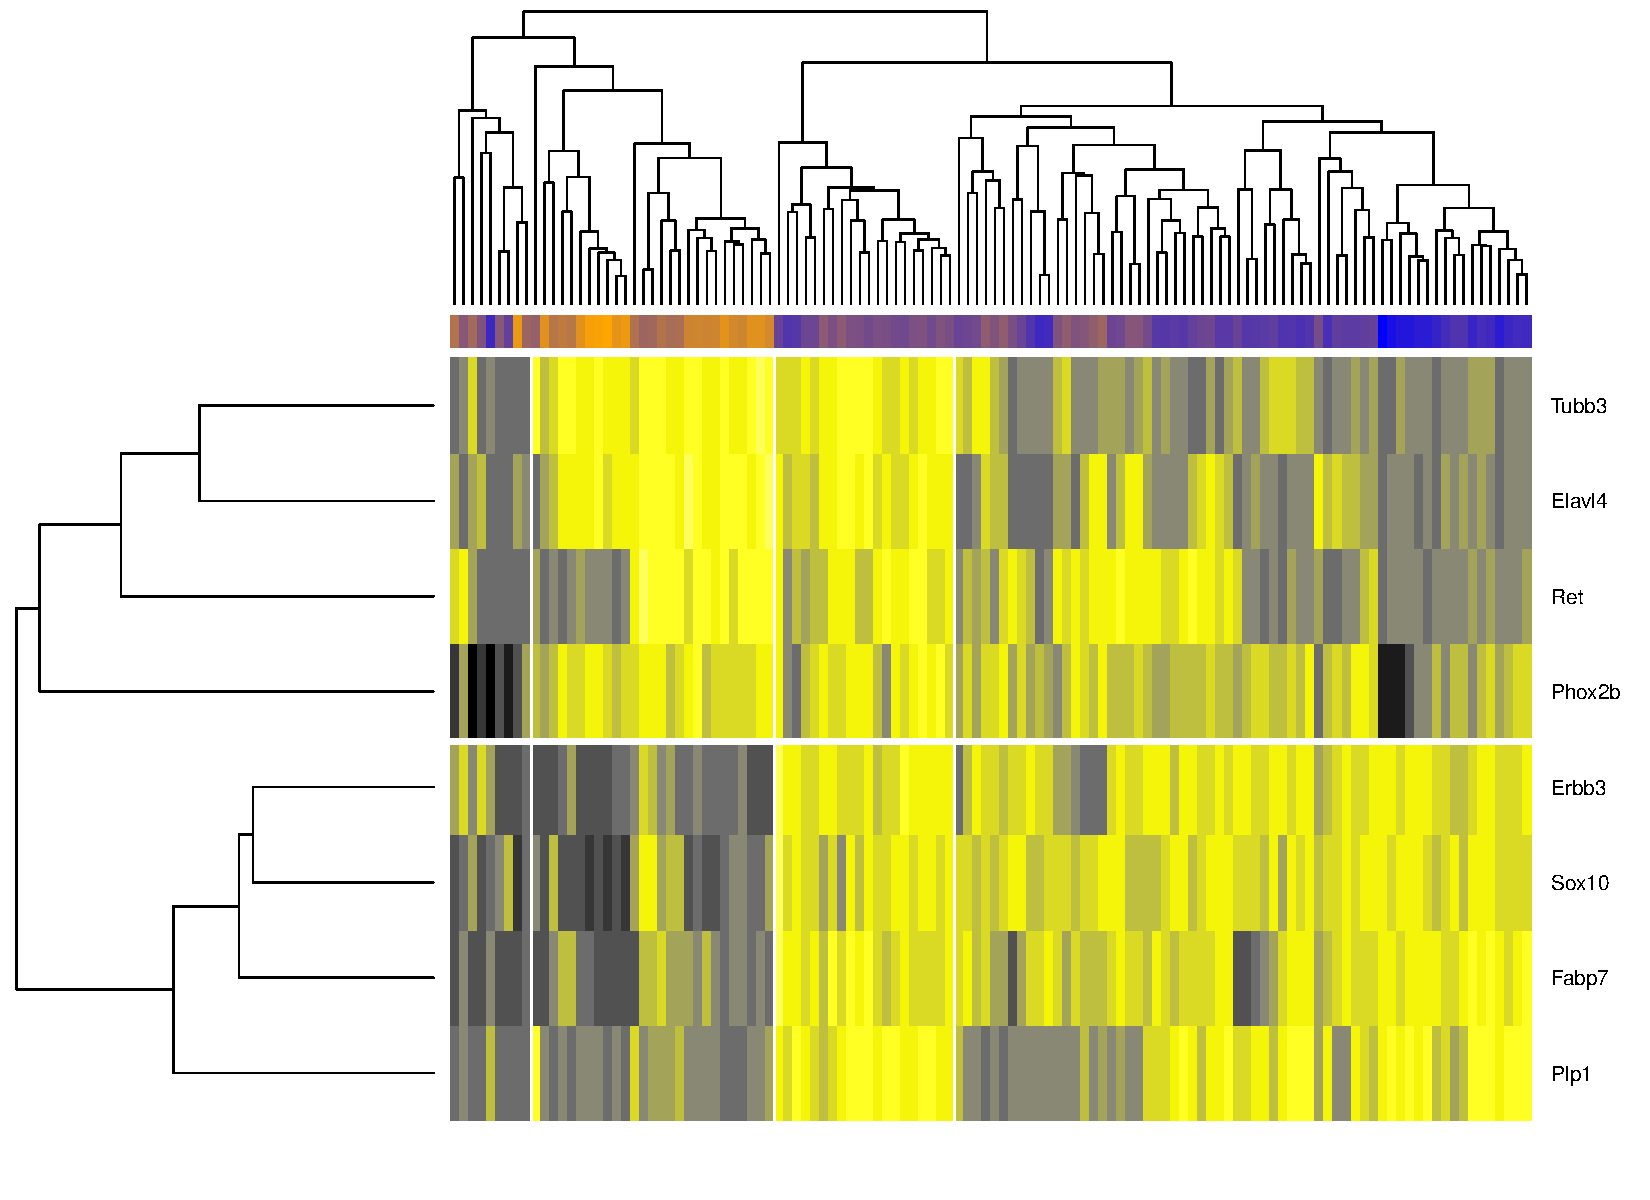
\includegraphics[width=1.0\textwidth]{./heatmap.pdf}
	\caption{Heatmap of single-cell marker gene expression.
			Cell lineages can be clearly identified through distinct
			glial and neuronal gene expression patterns.}
	\label{fig:heatmap}
\end{minipage}

\begin{figure}
\begin{minipage}{0.45\textwidth}
	\centering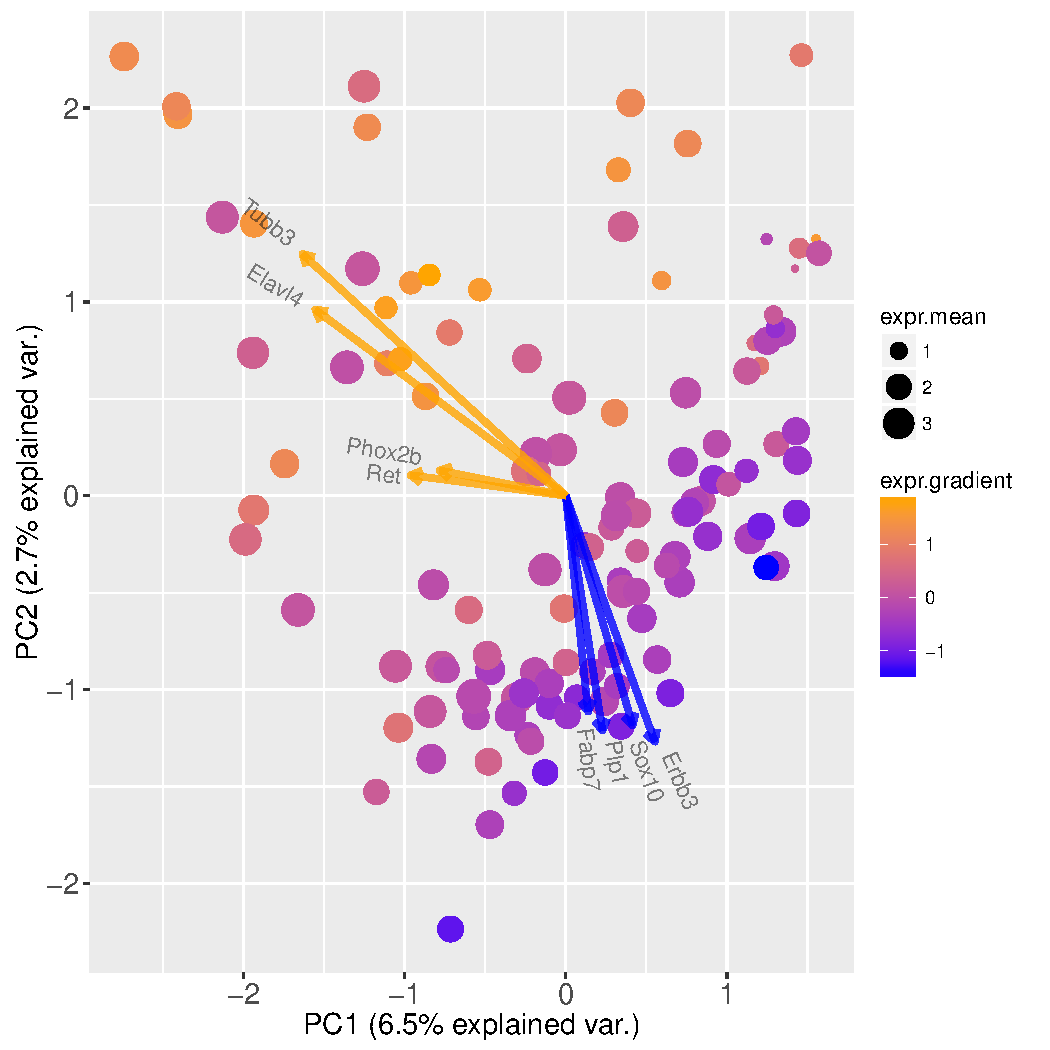
\includegraphics[width=1.0\textwidth]{./biplot_semisuperv.pdf}
	\caption{Biplot of single-cell gene expression. The underlying data set
		comprises the most divergently expressed genes. The gradient of marker
		expression is illustrated as colour shade beetween in blue (glial) and
		orange (neuronal).
		Total marker expression is indicated by the size of the sphere symbol.
		Arrows show the direction and magnitude of marker gene vectors
		in the given PC1/PC2 plane.}
	\label{fig:biplot}
\end{minipage}

%______________________________________________________________________________
\begin{myblock}{\sig{} Detection of Lineage-Specific Genes}
Using the expression profile of marker genes across all single-cells,
a linear regression model was applied and the resulting fit was assessed
by ANOVA. The set of best fitting genes is listed below for the neuronal
marker Tubb3 and the glial marker Erbb3.
\vspace{2cm}
\begin{figure}
\begin{minipage}{1.0\textwidth}
	\centering\includegraphics[width=0.7\textwidth]{./}
	\caption{Lists of genes with expression profiles similar to those of
			the neuronal marker Tubb3 (left) and Erbb3 (right).}
	\label{fig:genebars}
\end{minipage}
\end{figure}
\end{myblock}\vfill
%______________________________________________________________________________
}\end{minipage}
\end{beamercolorbox}
\end{column}

%______________________________________________________________________________
%______________________________________________________________________________
\begin{column}{.45\textwidth}
\begin{beamercolorbox}[center]{postercolumn}
\begin{minipage}{.98\textwidth}
\parbox[t][\columnheight]{\textwidth}{
%______________________________________________________________________________
\begin{myblock}{Cross-Sectional Time Series}

\begin{figure}
\begin{minipage}{1.0\textwidth}
	\centering\includegraphics[width=1.0\textwidth]{./}
	\caption{
			}
	\label{fig:timeseries}
\end{minipage}
\end{figure}
\end{myblock}\vfill
%______________________________________________________________________________
\begin{myblock}{Pseudotime Analysis}
The cross-sectional time series was further investigated by latent vaiable analysis,
where the latent variable was either a biological process (like 'cell cycle')
or the internal developmental time modeled as a 'pseudotime'.
Pseudotime estimation was performed by means of Gaussian Process Latent
Variable Modelling on the most divergent genes \cite{Reid_2016}.
The model has yielded ordering of single cells along the developmental
pseudotime line and accordingly expression profiles of genes that correlate with
lineage development in the ENS. The Bayesian model provides not only the most likely
posterior distribution, but also the associated uncertanties of the estimates.

\begin{figure}
\begin{minipage}{0.45\textwidth}
	\centering\includegraphics[width=1.0\textwidth]{./}
	\caption{.}
	\label{fig:pseudotime}
\end{minipage}
\end{figure}
\end{myblock}\vfill

%______________________________________________________________________________
\begin{myblock}{References}
\footnotesize
\bibliographystyle{abbrv}
\bibliography{./poster}
\end{myblock}\vfill
%______________________________________________________________________________
}\end{minipage}
\end{beamercolorbox}
\end{column}
%______________________________________________________________________________
\end{columns}
\end{frame}
\end{document}
%================================================================================

